\experiment{Binary Tree}{29/11/2023}

\section{Aim}
Implement binatry tree ADT with operations insertNode,preorder search, inorder search and postorder search.
\section{Algorithm}
 {\fontfamily{lmtt}\selectfont

  \begin{enumerate}[label=\arabic*.]
    \item Start

    \item Define a structure for a binary tree node:
          \begin{enumerate}[label=\arabic{enumi}.\arabic*.]
            \item Include data, left, and right pointers.
          \end{enumerate}

    \item Define a structure for a queue:
          \begin{enumerate}[label=\arabic{enumi}.\arabic*.]
            \item Include front, back, size, and an array of node pointers.
          \end{enumerate}

    \item Create a function to initialize a new queue:
          \begin{enumerate}[label=\arabic{enumi}.\arabic*.]
            \item Allocate memory for the queue.
            \item Set front and back to -1, and size to 100.
            \item Return the created queue.
          \end{enumerate}

    \item Create a function to enqueue a node into the queue:
          \begin{enumerate}[label=\arabic{enumi}.\arabic*.]
            \item Check if the queue is empty.
            \item If empty, set front and back to 0 and add the node to the array.
            \item If not empty, check for queue overflow.
            \item If no overflow, increment back and add the node to the array.
          \end{enumerate}

    \item Create a function to dequeue a node from the queue:
          \begin{enumerate}[label=\arabic{enumi}.\arabic*.]
            \item Check if the queue is empty.
            \item If empty, display "Queue underflow" and return NULL.
            \item If not empty, get the node at the front, update front.
            \item If front and back become equal, set them to -1.
          \end{enumerate}

    \item Create a function to insert a node into the binary tree:
          \begin{enumerate}[label=\arabic{enumi}.\arabic*.]
            \item Allocate memory for a new node and set its data.
            \item Check if the tree is empty.
            \item If empty, set the new node as the root and return.
            \item If not empty, create a queue and enqueue the root.
            \item Traverse the tree using the queue:
                  \begin{enumerate}[label=\arabic{enumi}.\arabic{enumii}.\arabic*.]
                    \item Dequeue a node and check its left and right children.
                    \item If left is NULL, insert the new node as the left child.
                    \item If right is NULL, insert the new node as the right child.
                    \item Enqueue non-null children for further exploration.
                  \end{enumerate}
          \end{enumerate}

    \item Create functions for preOrder, inOrder, and postOrder traversal:
          \begin{enumerate}[label=\arabic{enumi}.\arabic*.]
            \item Check if the current node is not NULL.
            \item Print the data of the current node.
            \item Recursively traverse the left subtree.
            \item Recursively traverse the right subtree.
          \end{enumerate}

    \item In the main function:
          \begin{enumerate}[label=\arabic{enumi}.\arabic*.]
            \item Initialize a root node as NULL.
            \item Create a loop to display a menu and perform operations based on user input.
            \item Inside the loop:
                  \begin{enumerate}[label=\arabic{enumi}.\arabic{enumii}.\arabic*.]
                    \item If the user chooses to insert a node, take input and call the insert function.
                    \item If the user chooses traversal options, call the corresponding traversal functions.
                  \end{enumerate}
            \item Continue the loop until the user chooses to exit.
          \end{enumerate}

    \item Stop
  \end{enumerate}

 }
\section{C Program}

\begin{lstlisting}[label={list:c_progam1:binary_tree}]
#include <stdlib.h>
#include <stdio.h>

typedef struct Node
{
  int data;
  struct Node *left;
  struct Node *right;
} node;

typedef struct queue
{
  int front;
  int back;
  int size;
  node *arr[100];
} queue;

// Queue
queue *createQueue();
void enqueue(queue *q, node *node);
node *dequeue(queue *q);

// Binary Tree
node *insert(node *root, int data);
void preorder(node *root);
void inorder(node *root);
void postorder(node *root);

int main()
{
  node *root = NULL;

  int ch;
  printf("1)Insert Node\n2)PreOrder Traversal\n3)InOrder Traversal\n4)PostOrder Traversal\n5)Exit");
  do
  {
    printf("\nChoice: ");
    scanf("%d", &ch);
    if (ch == 1)
    {
      int x;
      printf("\nEnter the data: ");
      scanf("%d", &x);
      root = insert(root, x);
    }
    else if (ch == 2)
    {
      printf("\nPreOrder: ");
      preorder(root);
      printf("\n");
    }
    if (ch == 3)
    {
      printf("\nInOrder: ");
      inorder(root);
      printf("\n");
    }
    else if (ch == 4)
    {
      printf("\nPostOrder: ");
      postorder(root);
      printf("\n");
    }
  } while (ch != 5);
}
queue *createQueue()
{
  queue *q = (queue *)malloc(sizeof(queue));
  q->front = -1;
  q->back = -1;
  q->size = 100;
  return q;
}

void enqueue(queue *q, node *node)
{
  if (q->front == -1 && q->back == -1)
  {
    q->front = 0;
    q->back = 0;
    q->arr[q->back] = node;
    return;
  }
  else if (q->back == q->size - 1)
  {
    printf("\nQueue overflow\n");
    return;
  }
  q->back++;
  q->arr[q->back] = node;
}

node *dequeue(queue *q)
{
  node *removed;
  if (q->back == q->front)
  {
    if (q->front == -1)
    {
      printf("\nQueue underflow!\n");
      return NULL;
    }
    removed = q->arr[q->front];
    q->front = -1;
    q->back = -1;
  }
  else
  {
    removed = q->arr[q->front];
    q->front++;
  }
  return removed;
}

node *insert(node *root, int data)
{
  node *new = (node *)malloc(sizeof(node));
  new->data = data;
  new->left = NULL;
  new->right = NULL;
  if (root == NULL)
  {
    root = new;
    return root;
  }
  queue *q = createQueue();
  enqueue(q, root);
  while (q->front != -1)
  {
    node *current = dequeue(q);
    if (current->left == NULL)
    {
      current->left = new;
      break;
    }
    else if (current->right == NULL)
    {
      current->right = new;
      break;
    }
    else
    {
      enqueue(q, current->left);
      enqueue(q, current->right);
    }
  }
  return root;
}

void preorder(node *root)
{
  if (root != NULL)
  {
    printf("%d, ", root->data);
    preorder(root->left);
    preorder(root->right);
  }
}

void inorder(node *root)
{
  if (root != NULL)
  {
    inorder(root->left);
    printf("%d, ", root->data);
    inorder(root->right);
  }
}

void postorder(node *root)
{
  if (root != NULL)
  {
    postorder(root->left);
    postorder(root->right);
    printf("%d, ", root->data);
  }
}
\end{lstlisting}


\section{Output}
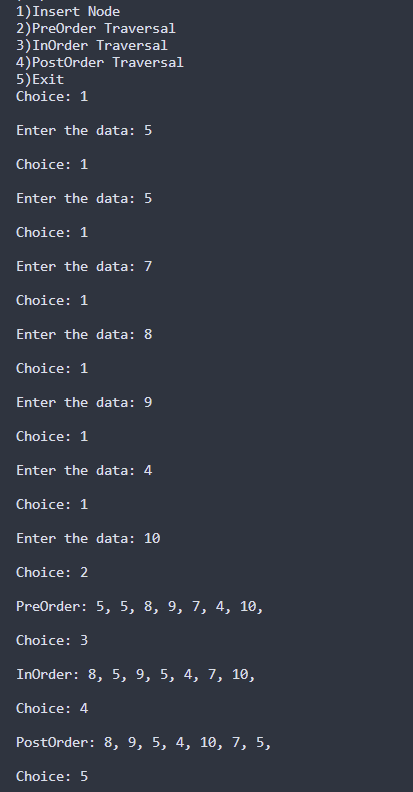
\includegraphics[]{Cycle_2/Outputs/BinaryTree.png}


\section{Result}
Program is executed successfully and output is verified.